\section{Cubic BaTiO$_3$}
\label{sec9:BaTiO3}

\begin{itemize}
	\item Outline : {\it Obtain MLWFs for a perovskite.}
\end{itemize}

\begin{figure}[h!]
\centering
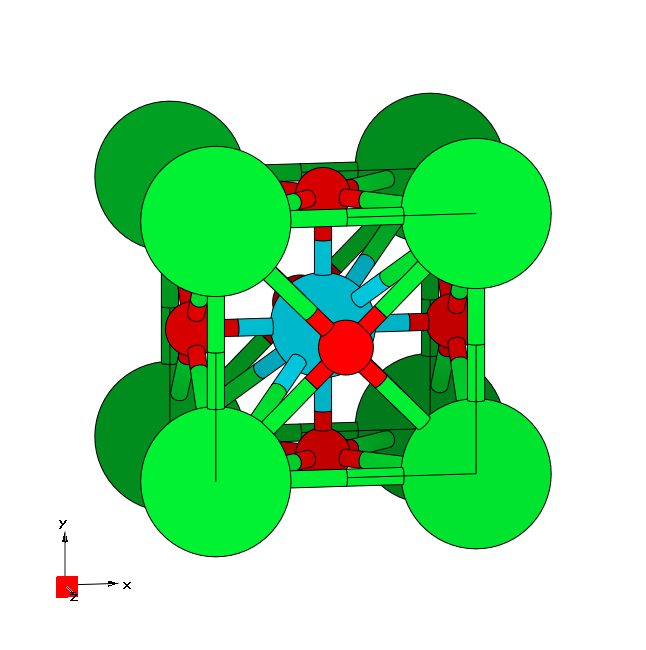
\includegraphics[width=0.25\columnwidth,trim={45pt 45pt 55pt 55pt},clip]{figure/example09/BaTiO3.png}
\caption{Unit cell of cubic BaTiO$_3$ crystal plotted with the \xcrysden{} program.}
\label{fig9.0}
\end{figure}

\begin{itemize}
	\item[1-5] {\it Compute the MLWFs.}

	Converged values for the total spread functional and its components are shown in Tab.~\ref{tab9.1}. 
\end{itemize}

\begin{table}[b!]
	\centering
	\captionsetup{width=.5\textwidth}
	\caption{Converged values of the components of spread functional and their sums for cubic BaTiO$_3$ in \angsqd{}.}
	\begin{tabular}{@{} lllll @{}}\toprule[1.5pt]
	$\Omega$ & $\Omega\tinysub{I}$ & $\Omega\tinysub{OD}$ & $\Omega\tinysub{D}$ & $N_{\mathrm{iter}}$ \\\midrule
	12.7187 & 12.5662 & 0.1525 &  0.000 & 50 \\\bottomrule[1pt]
	\end{tabular}\label{tab9.1}
\end{table} 

\begin{itemize}
	\item {\it Plot the second MLWF.}

	The result is shown in \Fig{fig9.1}-(a) and -(b). 
	\begin{figure}[h!]
	\centering
	\subfloat[top]{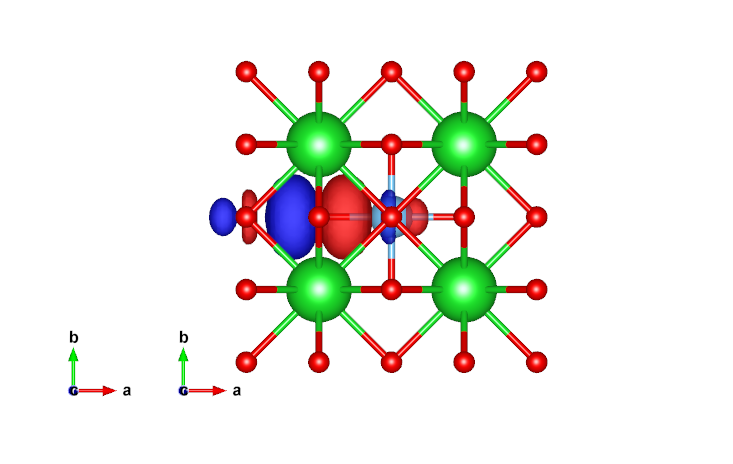
\includegraphics[width=0.35\columnwidth,trim={140pt 50pt 50pt 50pt},clip]{figure/example09/BaTiO3_00002_side.png}}
	\centering
	\subfloat[side]{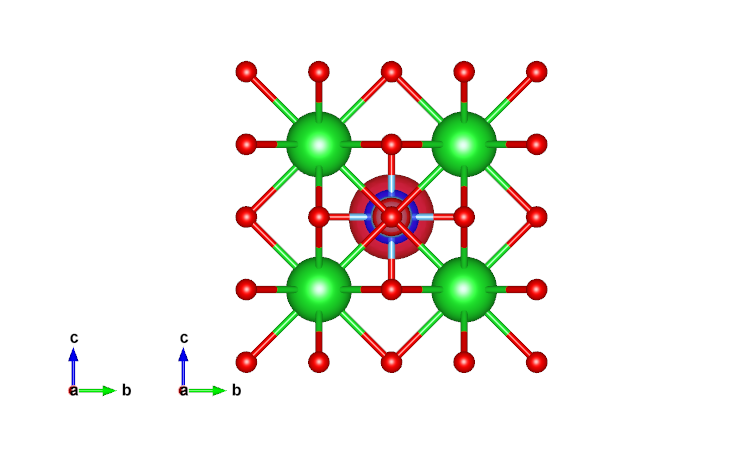
\includegraphics[width=0.35\columnwidth,trim={140pt 50pt 50pt 50pt},clip]{figure/example09/BaTiO3_00002_top.png}}
	\caption{Top-view (a) and side-view (b) of the second MLWF in BaTiO$_3$ }\label{fig9.1}
	\end{figure}


	\item {\it We can now simulate the ferroelectric phase by displacing the Ti atom. Regenerate the MLWFs (i.e., compute the ground-state charge density and Bloch states using pwscf, etc.) and look at the change in the second MLWF.}
	
	The result is shown in \Fig{fig9.2}-(a) and -(b).
	\begin{figure}[h!]
	\centering
	\subfloat[top]{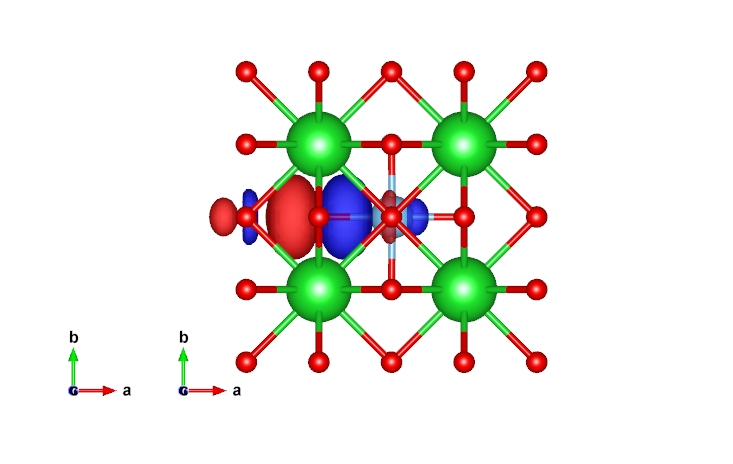
\includegraphics[width=0.35\columnwidth,trim={140pt 50pt 50pt 50pt},clip]{figure/example09/BaTiO3_00002_displaced.png}}
	\centering
	\subfloat[side]{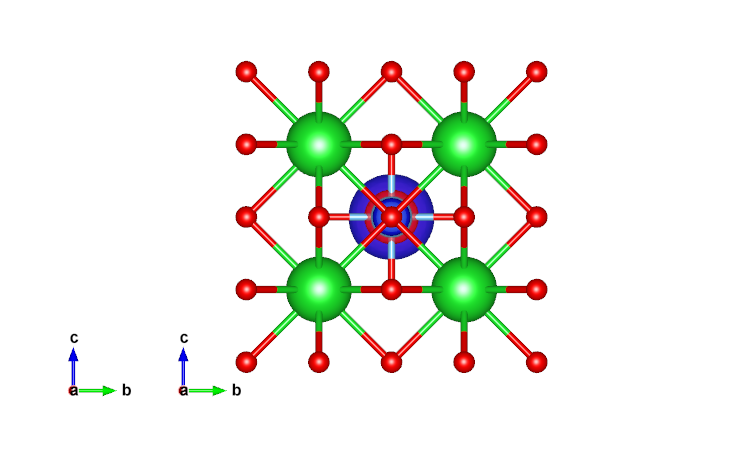
\includegraphics[width=0.35\columnwidth,trim={140pt 50pt 50pt 50pt},clip]{figure/example09/BaTiO3_00002_displaced_top.png}}
	\caption{Top-view (a) and side-view (b) of the second MLWF in BaTiO$_3$ with the Ti atom displaced.}\label{fig9.2}
	\end{figure}
\end{itemize}

\subsection*{Further ideas}
\begin{itemize}
	\item {\it Look at \MLWFs{} for other groups of bands.}

	Plots of MLWFs for other group of bands are shown in \Fig{fig9.3}-(a)-(b)-(c)-(d)-(e) and -(f). 
	\begin{figure}[t!]
	\centering
	\subfloat[Exclude bands = 2-20. \protect\\ Ti:s]{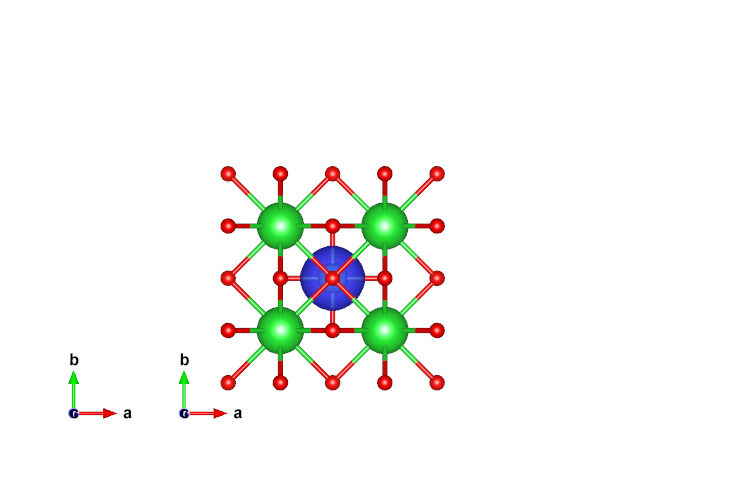
\includegraphics[width=0.3\columnwidth,trim={140pt 50pt 200pt 150pt},clip]{figure/example09/BaTiO3_Ti_3s.png}}
	\centering
	\subfloat[Exclude bands = 1,5-20. \protect\\ Ti:p]{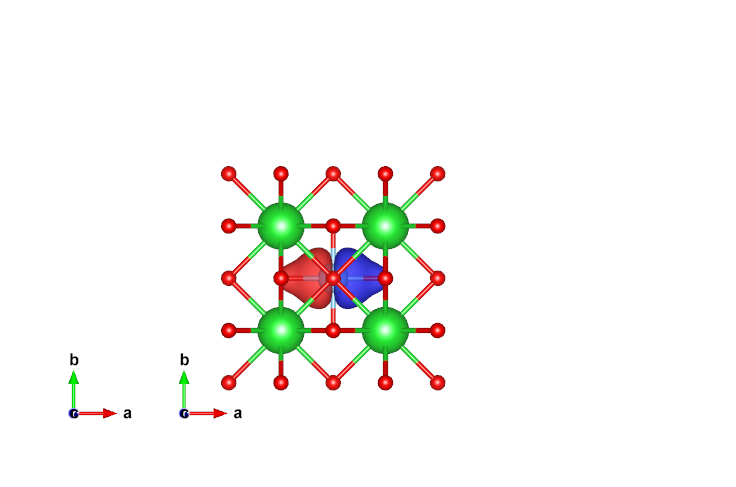
\includegraphics[width=0.3\columnwidth,trim={140pt 50pt 200pt 150pt},clip]{figure/example09/BaTiO3_Ti_3p.png}}
	\centering
	\subfloat[Exclude bands = 1-4,6-20. \protect\\ Ba:s]{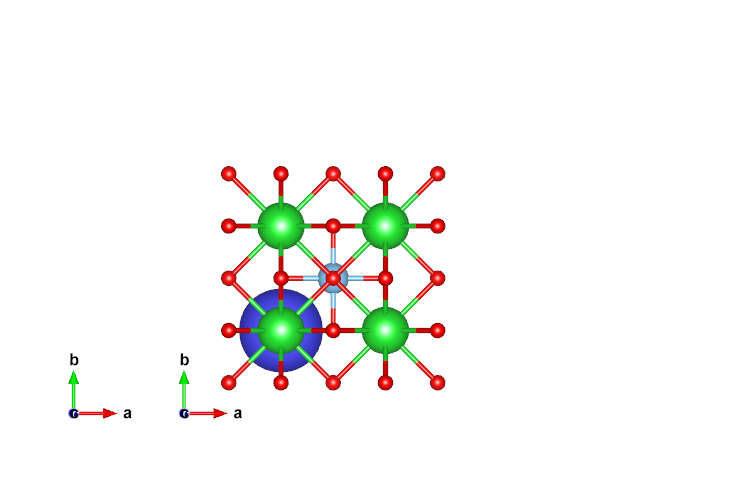
\includegraphics[width=0.3\columnwidth,trim={140pt 50pt 200pt 150pt},clip]{figure/example09/BaTiO3_Ba_5s.png}}\\
	\centering
	\subfloat[Exclude bands = 1-5,9-20. \protect\\ O:s]{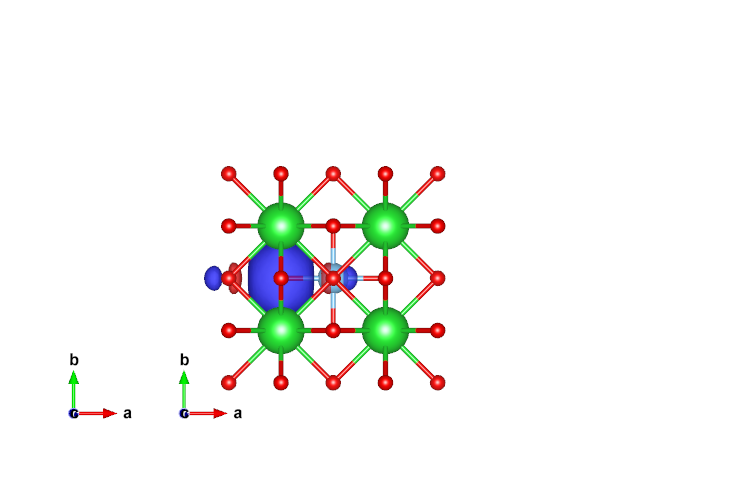
\includegraphics[width= 0.3\columnwidth,trim={140pt 50pt 200pt 150pt},clip]{figure/example09/BaTiO3_O_2s.png}}
	\centering
	\subfloat[Exclude bands = 1-8,12-20. \protect\\ Ba:p]{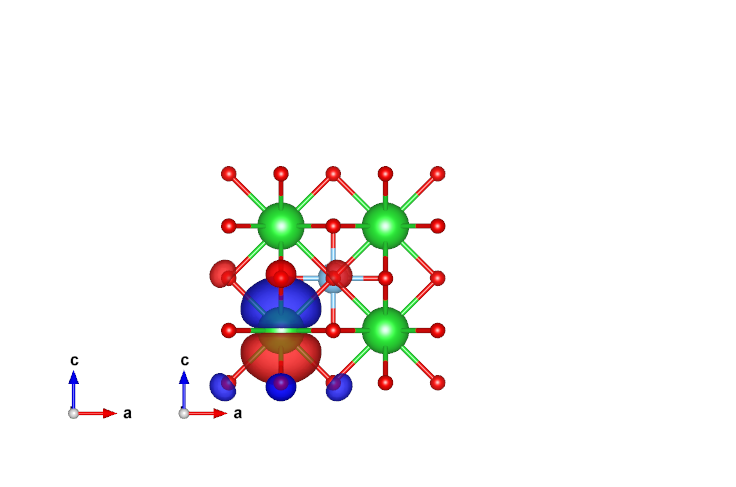
\includegraphics[width=0.3\columnwidth,trim={140pt 50pt 200pt 150pt},clip]{figure/example09/BaTiO3_Ba_5p.png}}
	\centering
	\subfloat[Exclude bands = 1-11. \protect\\ O:p]{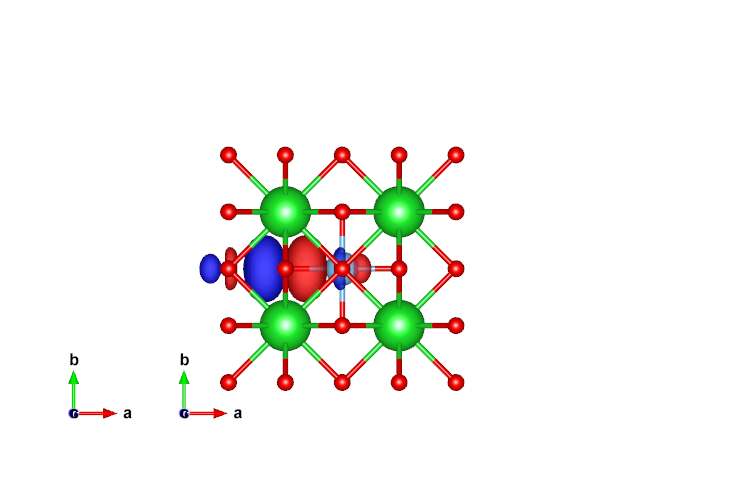
\includegraphics[width= 0.3\columnwidth,trim={140pt 50pt 170pt 130pt},clip]{figure/example09/BaTiO3_O_2p.png}}
	\caption{\MLWFs{} for other group of bands.}\label{fig9.3}
	\end{figure}

    \item {\it What happens if you form MLWFs for the whole valence manifold?}

    Some representative \MLWFs{} from the wannierisation of the whole valence bands are shown in \Fig{fig9.4}.
	\begin{figure}[b!]
	\centering
	\subfloat[Ti $3s$]{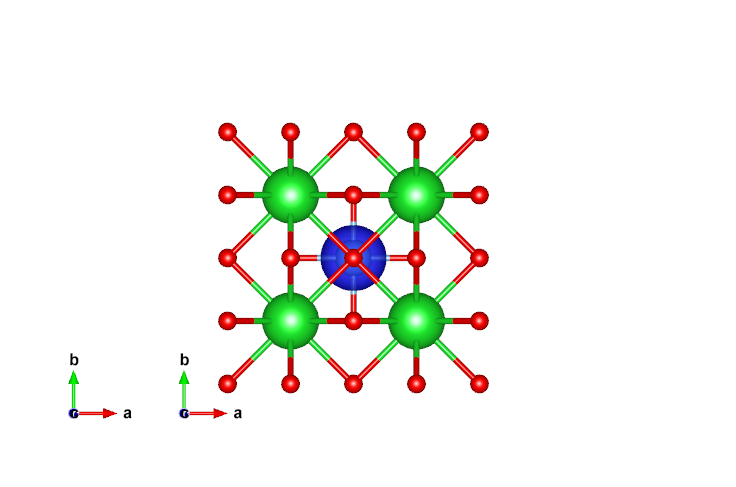
\includegraphics[width=0.3\columnwidth,trim={140pt 50pt 150pt 100pt},clip]{figure/example09/BaTiO3_Ti_3s_valence.png}}
	\centering
	\subfloat[Ti $3p$]{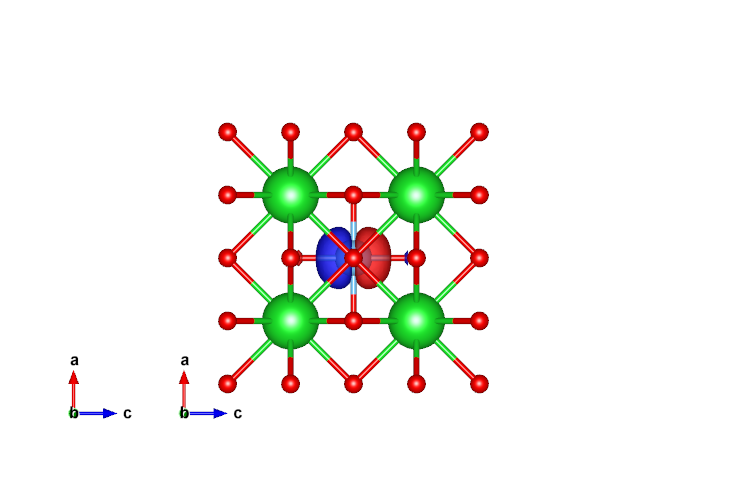
\includegraphics[width=0.3\columnwidth,trim={140pt 50pt 150pt 100pt},clip]{figure/example09/BaTiO3_Ti_3p_valence.png}}
	\centering
	\subfloat[Ba $5s$]{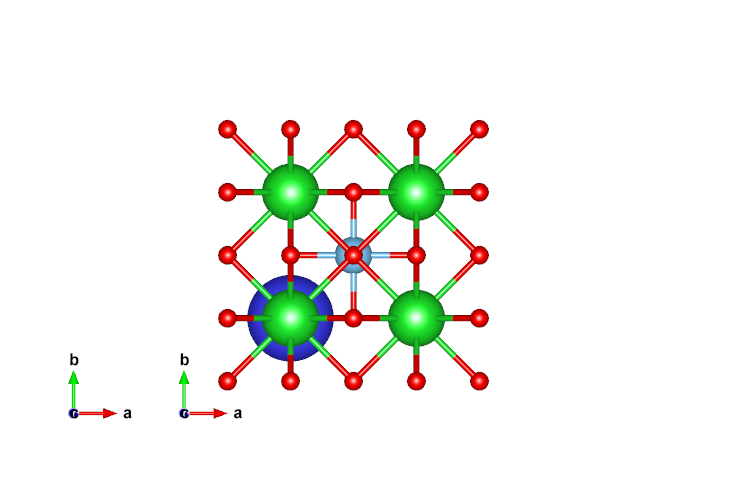
\includegraphics[width=0.3\columnwidth,trim={140pt 50pt 150pt 100pt},clip]{figure/example09/BaTiO3_Ba_5s_valence.png}}\\
	\centering
	\subfloat[O $2s$]{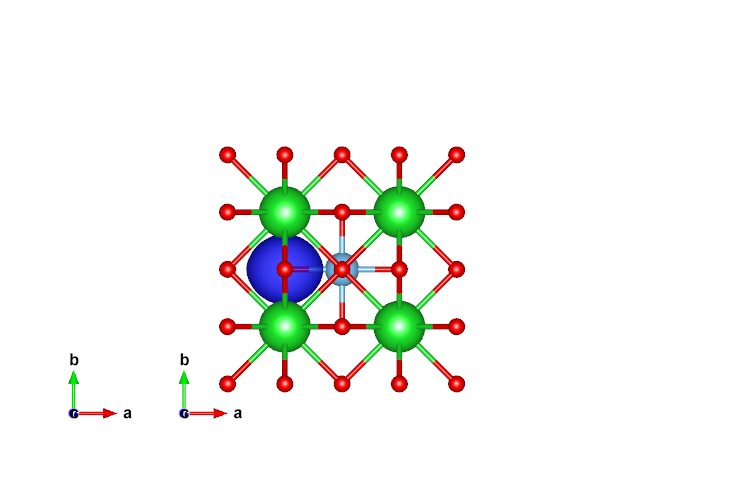
\includegraphics[width= 0.3\columnwidth,trim={140pt 50pt 150pt 100pt},clip]{figure/example09/BaTiO3_O_2s_valence.png}}
	\centering
	\subfloat[Ba $5p$]{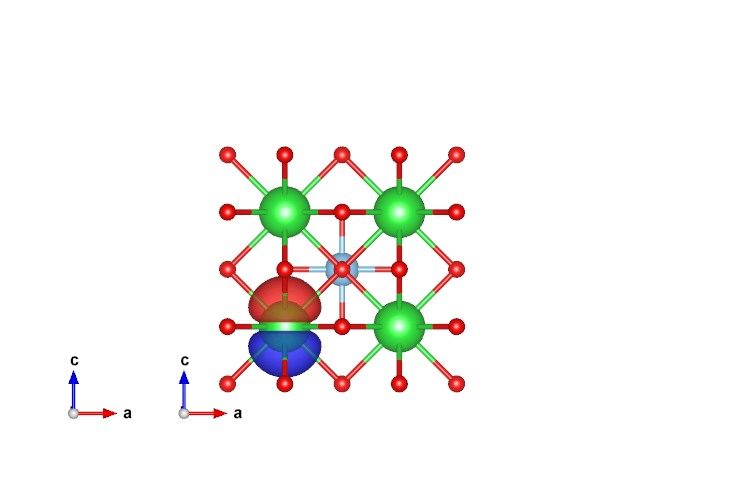
\includegraphics[width=0.3\columnwidth,trim={140pt 50pt 150pt 100pt},clip]{figure/example09/BaTiO3_Ba_5p_valence.png}}
	\centering
	\subfloat[O $2p$]{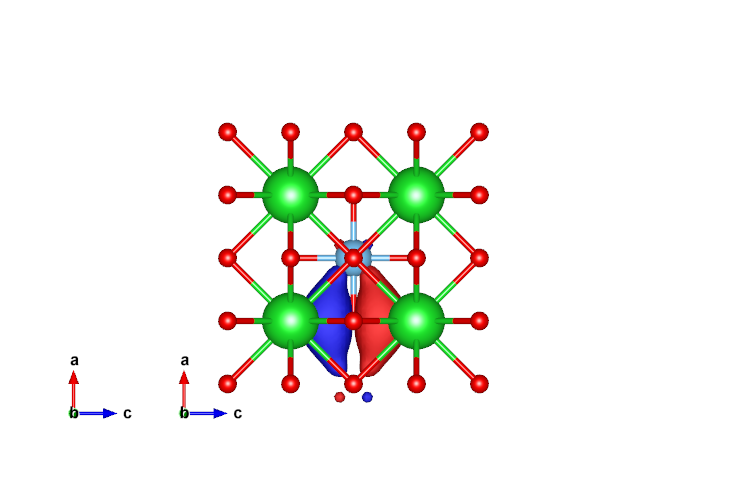
\includegraphics[width= 0.3\columnwidth,trim={140pt 50pt 150pt 100pt},clip]{figure/example09/BaTiO3_O_2p_valence.png}}
	\caption{\MLWFs{} formed from the whole valence manifold, i.e. from 20 bands.}\label{fig9.4}
	\end{figure}
\end{itemize}
